%%%%%%%%%%%%%%%%%%%%%%%%%%%%%%%%%%%%%%%
% Ch3 : Introduction to heat transfer %
%%%%%%%%%%%%%%%%%%%%%%%%%%%%%%%%%%%%%%%

\chapter{Heat tranfer}
\section{Introduction}
	We retrieve heat transfer in many phenomena like the combustion of coal that we use for the barbecue, the steel production or in power plants. But thermodynamics don't tell us how fast combustion will take place, chemistry tells us it will go too fast and each reaction needs its own reaction rate. \\
	Heat transfer is important in the duration of many processes. It's important to design and understand that principle for engineers. 
	
	\subsection{Definitions}
	\subsubsection{Energy}
		\begin{center}
		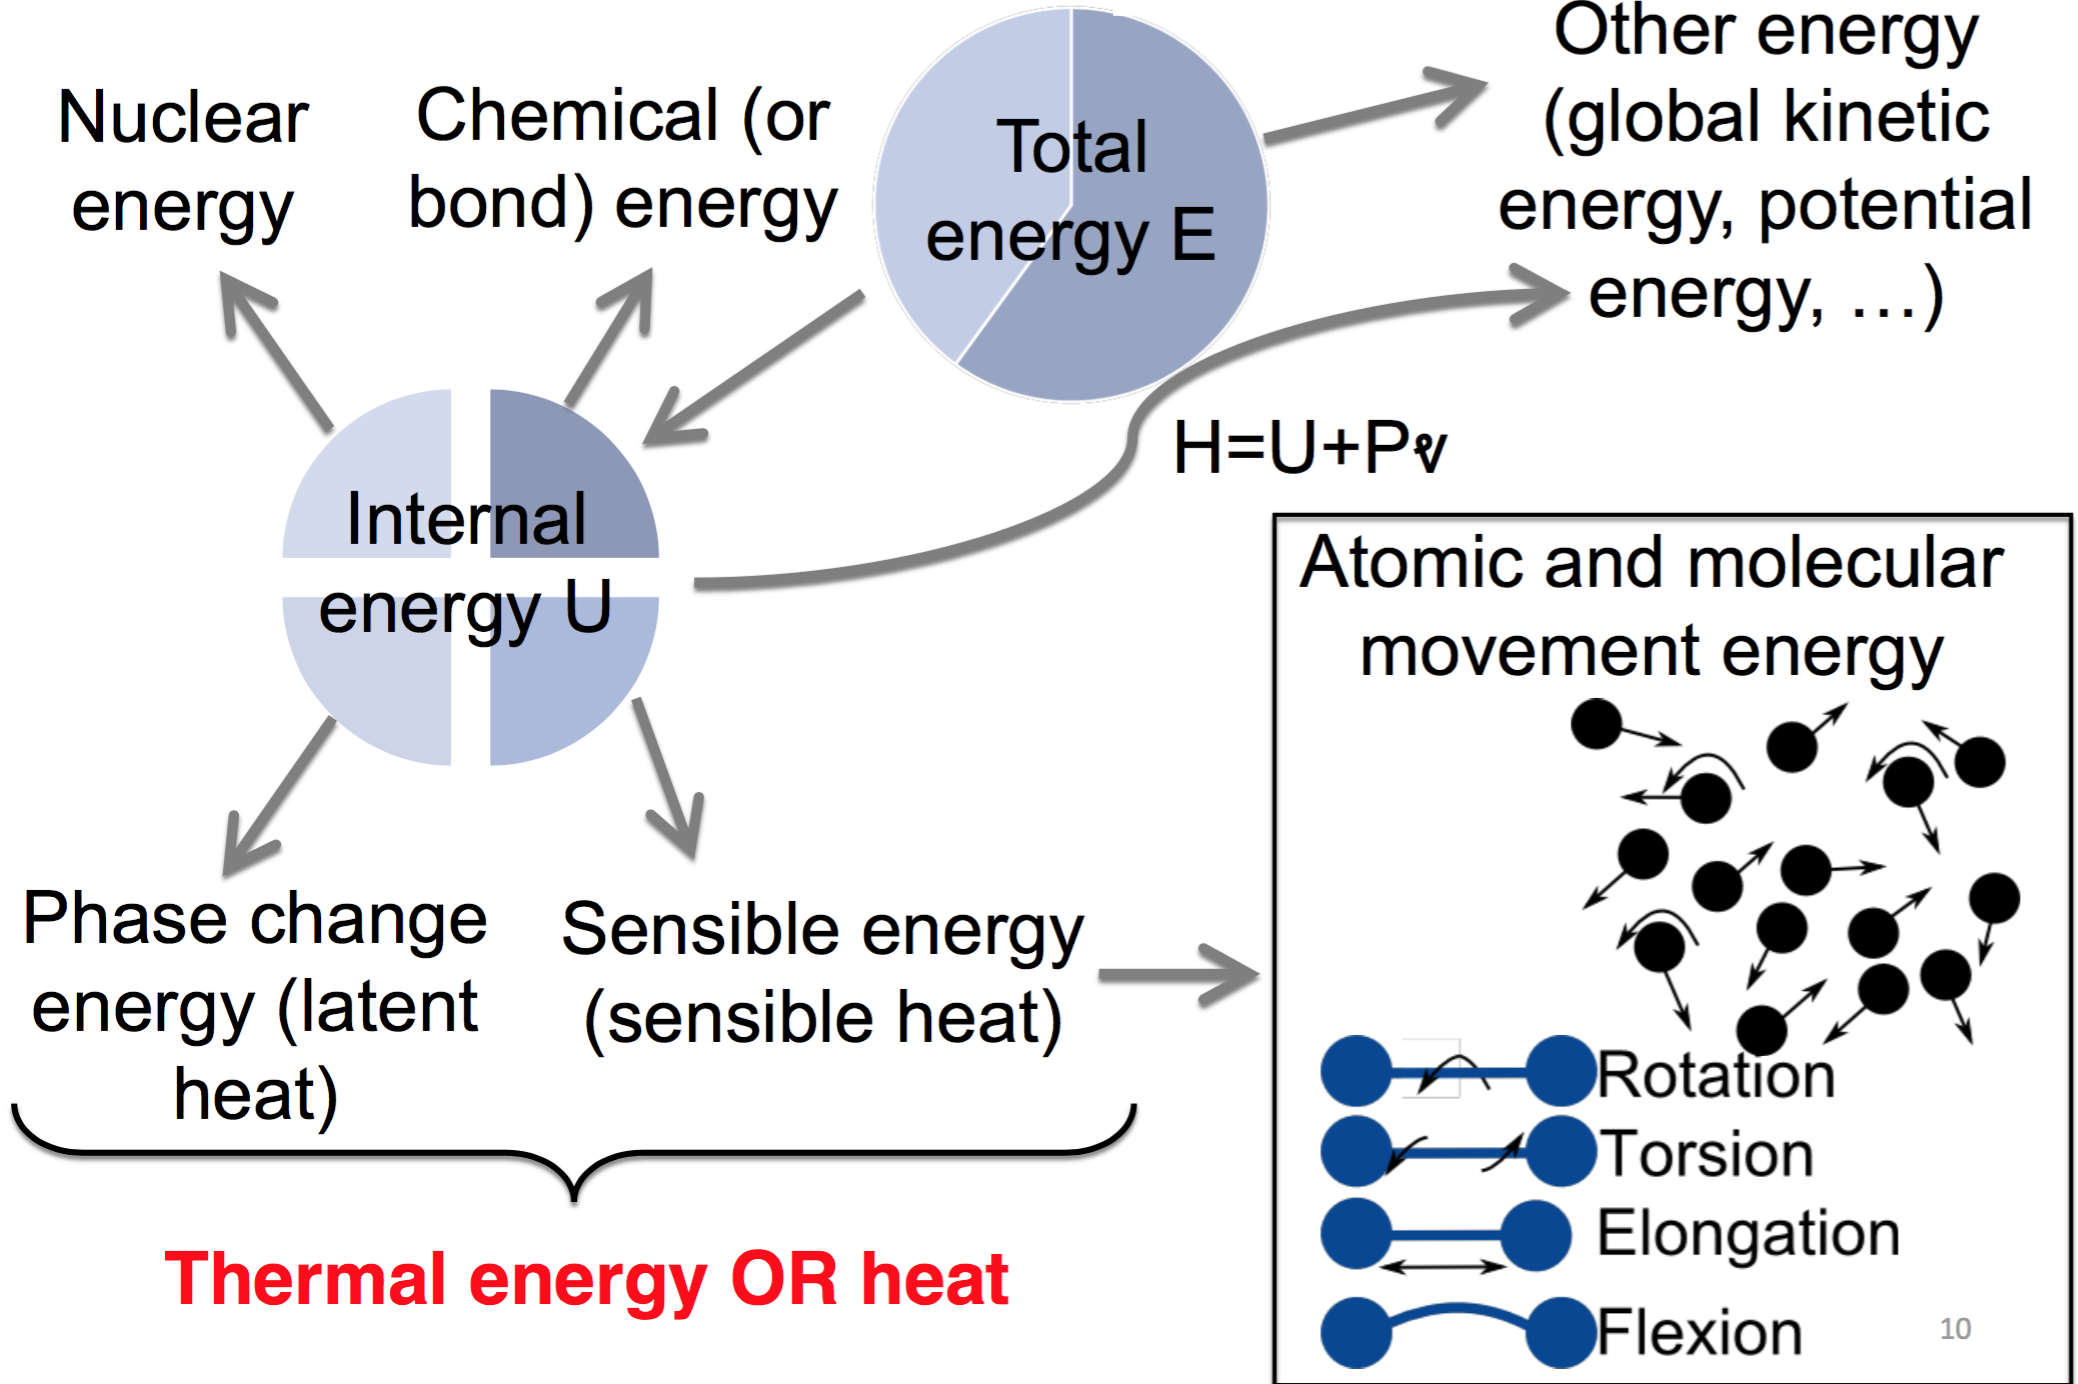
\includegraphics[scale=0.25]{ch3/1}
		\end{center}
		In a system you have the total energy and is divided in two : internal energy and the rest. The first is the energy you find in the system if you attach yourself to the system. Thermal energy or heat includes the \textbf{latent heat} that is the phase change energy and the \textbf{sensible heat} that is associated to the atomic move inside the material. 
		
	\subsubsection{Temperature}
		It's an interesting principle because it’s not simple to define it. You can have thermodynamic definition of temperature : linked to the entropie (system is changing) and microscopic theory linked to the move of particles. \\
		The important for us is that temperature is an intensive quantity correlated to the internal energy of the system. It’s a universal feature of matters so it’s independent of the material. \\
		Temperature is linked to the system energy by the specific heat 
		\begin{equation}
			dU = mc_v dT \qquad and \qquad dH = mc_p dT
		\end{equation}

		Should remember that gas of low pressure and low velocity can be considered as incompressible. In that case 
		\begin{equation}
			c_v = c_p = c
		\end{equation}		 
		
	\subsubsection{Heat flux}
		With 2 body at different temperatures in contact, a quantity $Q(J)$ of heat is transfered through a surface of area $A$. Heat transfer rate and heat transfer flux density are defined as 
		\begin{equation}
			\dot{Q} = \frac{dQ}{dt} \qquad \Rightarrow \qquad \dot{q} = \frac{\dot{Q}}{A}
		\end{equation}
		
\subsection{Heat balance}
		The idea is to see what heat induct. Heat is just a part of energy in the system, only the total energy is conserved. What we will do is make balances on a control volume but we will divide the energy in two parts (heat and the rest). We will take into account the heat flux entrance and exit on a control volume surface, the generation or the consumption and the accumulation :
		\begin{equation}
			\mbox{accumulation} + \mbox{out fluxes} + \mbox{sinks} = \mbox{sources} + \mbox{in fluxes}
		\end{equation}
		Sources and sinks can be due to the transformation of heat energy into a non thermal energy (sinks) or vice versa (source). \\
		We can divide the situation in 2. The one where we accumulate and the other where we don’t. The first case corresponds to stationary systems. The difference between \textbf{stationnary }and \textbf{equilibrium} is that the second is a particular stationary states where we have no flux whereas they are present in a stationnary flux. 

 \subsection{Heat transfer mechanisms}
 	\subsubsection{Conduction}
 		Universal heat transfer by contact. It appears in matter when molecules enter in contact with each others and tranfer heat. The entropic transport of heat is quite slow. Universal because it can happen everywhere we have matter and is the main heat transfer. Solid materials are caracterized as good heat conductor or not, so it's a material property.
 
 	\subsubsection{Convection}
 		\begin{wrapfigure}[5]{r}{1cm}
 		\vspace{-5mm}
 		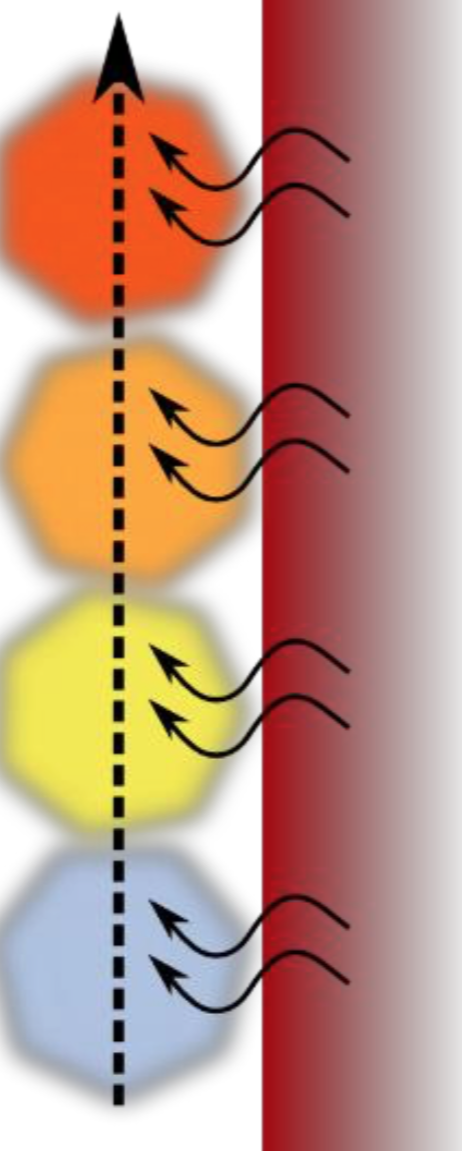
\includegraphics[scale=0.15]{ch3/2}
 		\end{wrapfigure}
		Convection is linked to the movement of the particles but they carry they own heat. During this movement conduction occurs : convection = conduction + advection (illustrated on the picture). It's the major tranfer in presence of flows. Convection is complicated, it depends on how moves the fluid, its direction, ...